
\documentclass[ms.tex]{subfiles}
\begin{document}

\section{Nucleosynthesis}
\label{sec:yields}

Here we make use of the chemical evolution model for the Milky Way
presented in~\citet{Johnson2021}, which runs using the publicly available
\texttt{Versatile Integrator for Chemical Evolution}
(\vice, see Appendix~\ref{sec:vice};~\citealp{Johnson2020, Griffith2021a,
Johnson2021}), an open-source~\python~package designed for GCE modeling.
\citet{Johnson2021} focus their discussion of the model predictions on O and
Fe, and we retain their yields of these elements here.
As required by~\vice, the SN yields are defined as the net mass of some element
X produced over all explosion events in units of the progenitor cluster's
mass.
For example, with a yield of~$y_\text{X} = 0.001$, a hypothetical~$1000~\msun$
star cluster would produce~$1~\msun$ of the element X instantaneously in the
case of core collapse supernovae (CCSNe) or over the delay-time distribution
(DTD) in the case of SNe Ia.
These yields are net yields in that they do not quantify the metal mass
ejected to the interstellar medium (ISM) that was initially present within a
star; in the previous example, the~$1~\msun$ yield is only the newly produced
metal mass.
We adopt the following values from~\citet{Johnson2021}, who in turn base them
off of~\citet*{Weinberg2017} and~\citet{Johnson2020}:
\begin{itemize}
	\item $\ycc{O} = 0.015$

	\item $\ycc{Fe} = 0.0012$

	\item $\yia{O} = 0$

	\item $\yia{Fe} = 0.00214$,
\end{itemize}
where the subscripts and superscripts differentiate between the element and the
SN type.
We explore variations of these values in the context of the overall
normalization of nucleosynthetic yields and Galactic outflows
in~\S~\ref{sec:results:yields}.
We assume that N is not produced in significant amounts by SNe Ia
\citep{Johnson2019}, seting~$\yia{N} = 0$ throughout this paper
accordingly, and spend the remainder of this section discussing the CCSN and
AGB star yields of N.
\par
A significant portion of N yields arise as a consequence of the CNO
cycle.\footnote{
	\Ctwelve(p,~$\gamma$)\Nthirteen($\beta^+~\nu_\text{e}$)\Cthirteen
	(p,~$\gamma$)\Nfourteen(p,~$\gamma$)\Ofifteen($\beta^+~\nu_\text{e}$)
	\Nfifteen(p,~$\alpha$)\Ctwelve
}
As the dominant source of pressure and energy in non-zero metallicity stars
with initial masses of~$\gtrsim$1.3~\msun, this cyclic nuclear reaction
catalyses the conversion of H into He that would otherwise be accomplished by
the proton-proton chain~\citep*{Suliga2021}.
Its slowest component by far is the~\Nfourteen(p,~$\gamma$)\Ofifteen~reaction
\citep[e.g.][]{LUNA2006}.
Consequently, the first order effect of the CNO cycle is to convert all of the
C and O isotopes in stellar cores into~\Nfourteen.
As we will discuss in this section, this plays an important role in shaping N
yields from stars of all masses.

\subsection{Core Collapse Supernovae and Massive Star Winds}
\label{sec:yields:ccsne}

In~\vice, CCSN nucleosynthetic products are approximated to be produced
instantaneously following an episode of star formation; this is a valid
approximation due to how short the lives of massive stars are compared to the
relevant timescales for GCE.
Based on this and its definition as being in units of a stellar population's
total mass, the yield is simply the constant of proportionality between the
CCSN production rate and the star formation rate (SFR):
\begin{equation}
\dot{M}_\text{X}^\text{CC} = \ycc{X}\dot{M}_\star
\end{equation}
More generally,~\ycc{X}~quantifies~\textit{all} of the nucleosynthetic material
approximated to be produced instantaneously following a single stellar
population's formation.

% fig 2
\begin{figure*}
\centering
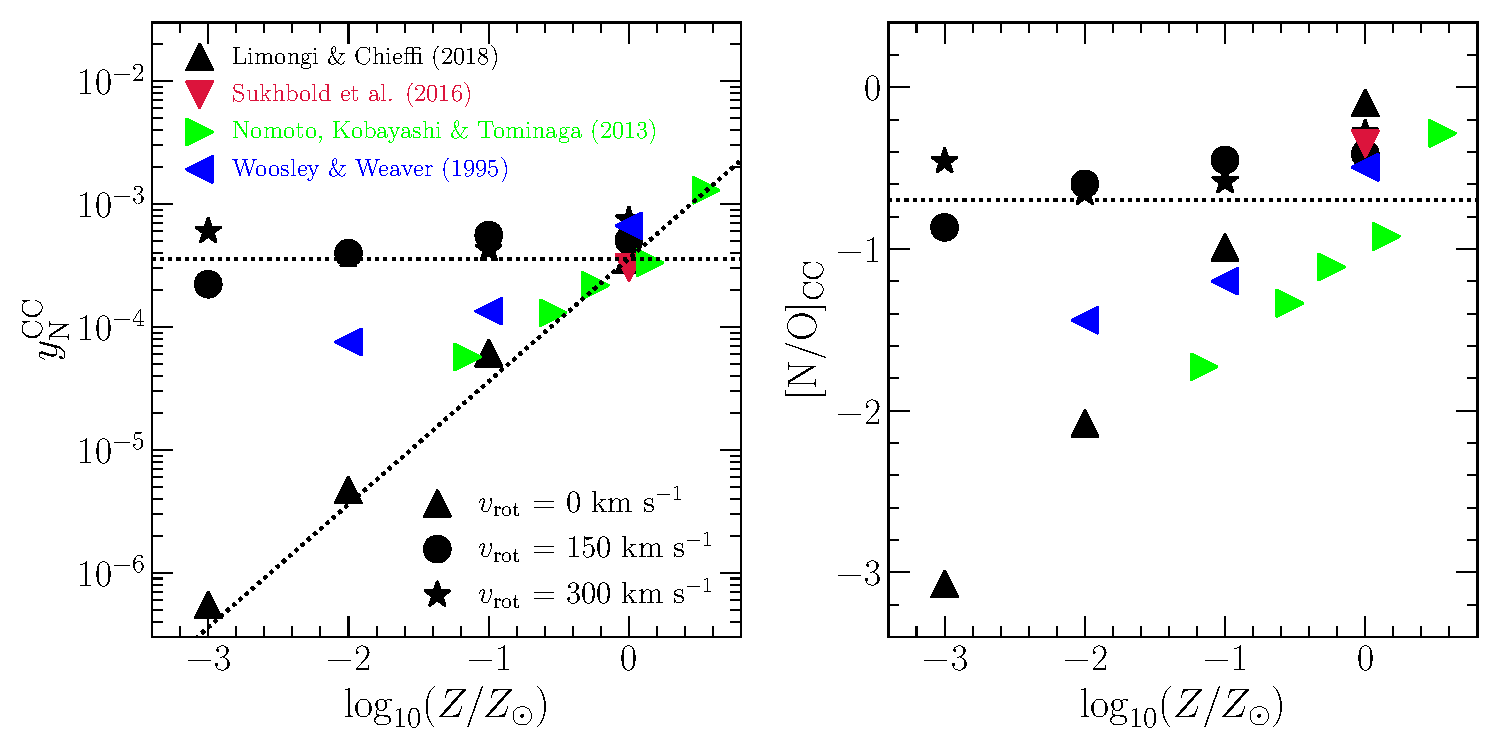
\includegraphics[scale = 0.63]{n_cc_yields.pdf}
\caption{
\textbf{Left}: IMF-averaged CCSN yields of N calculated using~\vice's
\texttt{vice.yields.ccsne.fractional} function with the tables published by
\citet[][blue]{Woosley1995},~\citet[][green]{Nomoto2013},
\citet[][red]{Sukhbold2016}, and~\citet[][black]{Limongi2018}.
All studies report yields for non-rotating progenitors, shown by the triangles;
for visual clarity, the triangles point in a different direction for each study
according to the legend.
\citet{Limongi2018} report additional yields for progenitors with rotational
velocities of 150 (circles) and 300 km/s (stars).
The horizontal dashed line markes~$\ycc{N} = 3.6\times10^{-4}$,
the value of our fiducial CCSN yield of N in our GCE models.
We use the form shown by the slanted line (equation X) in~\S~X in combination
with some of our AGB star yield models discussed in~\S~\ref{sec:yields:agb}.
\textbf{Right}: The~\no~ratio predicted by each of the explosion models in
the left-hand panel, under the same colour-coding and marker scheme.
We mark the position of~$\no = -0.7$ with a black dotted line, the value
roughly suggested by the observations of low-metallicity systems highlighted
in Fig.~\ref{fig:no_oh_observed}.
}
\label{fig:n_cc_yields}
\end{figure*}

We compute theoretically predicted values of~\ycc{N}~using
\vice's~\texttt{vice.yields.ccsne.fractional} function assuming a
\citet{Kroupa2001} IMF; details on how~\vice~handles these calculations can be
found in~\S~4 of~\citet{Griffith2021a} and in the~\vice~science 
documentation\footnote{\url
	{https://vice-astro.readthedocs.io/en/latest/science_documentation/yields}
}.
In the left panel of Fig.~\ref{fig:n_cc_yields}, we plot the results as a
function of progenitor metallicity as predicted by the~\citet{Woosley1995},
\citet*{Nomoto2013},~\citet{Sukhbold2016}, and~\citet{Limongi2018} tables.
There is good agreement between the various non-rotating models, but only
\citet{Limongi2018} report yields for progenitors with non-zero rotational
velocities; these yields are substantially larger than their non-rotating
counterparts, especially at low metallicity.
With few seed nuclei for the CNO cycle at low~$Z$, production of~\Nfourteen~is
difficult.
Rotation-induced mixing, a highly uncertain process~\citep{Zahn1992, Maeder1998,
Lagarde2012}, could transport newly produced C and O into the hydrogen burning
shell of the CCSN progenitor, facilitating~\Nfourteen~production
(\citealp{Frischknecht2016}; see also discussion in~\S~4.2 of
\citealp{Andrews2017}).
Consequently, N yields at low metallicity are quite sensitive to model-dependent
assumptions regarding stellar rotation and internal mixing processes
\citep{Heger2010}.
\par
We compute the~\no~ratio of CCSN ejecta from the values
of~\ycc{N}~and~\ycc{O}~predicted by a given yield table according to
\begin{equation}
\no\subcc = 
\log_{10}\left(\frac{\ycc{N}}{\ycc{O}}\right) -
\log_{10}\left(\frac{Z_{\text{N},\odot}}{Z_{\text{O},\odot}}\right),
\label{eq:no_subcc}
\end{equation}
where~$Z_{\text{X},\odot}$ is the abundance by mass of some element X in the
sun, for which we take~$Z_{\text{N},\odot} = 6.91\times10^{-4}$ and
$Z_{\text{O},\odot} = 5.72\times10^{-3}$ based on the photospheric measurements
of~\citet{Asplund2009}.
For each value of~\ycc{N}~in the left panel of Fig.~\ref{fig:n_cc_yields}, we
compute the corresponding values of~\ycc{O}~and illustrate the
resultant~\no\subcc~ratios in the right panel.
These yield ratios follow similar trends with progenitor metallicity and
rotation as~\ycc{N}~itself, a consequence of the fact that these
studies predict relatively metallicity- and rotation-independent O yields.
If we assume~\no\subcc~=~$-0.7$ as suggested by Fig.~\ref{fig:no_oh_observed}
and our adopted O yield of~$\ycc{O} = 0.015$, equation~\refp{eq:no_subcc}
suggests that~$\ycc{N} = 3.6\times10^{-4}$.
We highlight both~\no\subcc~=~$-0.7$ and~$\ycc{N} = 3.6\times10^{-4}$ with
horizontal black dashed lines in Fig.~\ref{fig:n_cc_yields}, finding good
agreement with the rotating progenitor models of~\citet{Limongi2018} in both
panels.
This suggests that rotating massive stars play an important role in
establishing N abundances at low metallicity as recently suggested by
\citet{Grisoni2021}.
We therefore take~$\ycc{N} = 3.6\times10^{-4}$ as our fiducial CCSN yield of N;
both the normalization and metallicity-independence of this choice are
supported by the~\citet{Limongi2018} models.
\par
The~\citet{Sukhbold2016} tables agree nearly perfectly with our empirical value
of~$\ycc{N} = 3.6\times10^{-4}$, but they overpredict~\no\subcc~by~$\sim$0.2
dex.
This is a consequence of the failed supernovae incorporated into their model
and the lowered values of~\ycc{O} that result (see discussion
in~\S~\ref{sec:results:yields}).
While N emerges in substantial amounts in winds, much of the O produced by
massive stars is ejected during the explosion, making the O yield more
sensitive to the black hole landscape~\citep{Griffith2021a}.
Although most of the SN models plotted in Fig.~\ref{fig:n_cc_yields} slightly
overestimate our empirical value of~\no\subcc~=~$-0.7$, they still fall short
of solar.
This implies the need for an additional enrichment channel, which is expected
because it is well understood that N is also produced in considerable amounts
by AGB stars~\citep{Johnson2019}.
Although our empirically calibrated N yield agrees well with
the~\citet{Limongi2018} predictions, massive star nucleosynthesis models
overwhelmingly neglect the impact of a potential binary companion,
and~\citet{Limongi2018} is no exception.
\citet{Farmer2021} recently investigated the impact of binary star evolution on
theoretically predicted yields and found a considerable increase in C
production.
Despite being an interesting possibility, GCE models with such yields are beyond
the scope of this paper.


\subsection{Asymptotic Giant Branch Stars}
\label{sec:yields:agb}

Similar to SNe,~\vice~requires AGB star yields to be parameterized as
fractional net yields.
For a yield~$\yagb{X}$, the mass yield is given by~$M_\star \yagb{X}$.
Enrichment proceeds as it does in~\citet{Johnson2021} under the caveat that
AGB stars place their nucleosynthetic products in the~$\delta\rgal = 100$ pc
ring that they are in at a given time, allowing stars to enrich distributions
of radii as they migrate.
In short,~\vice~implements an algorithm which computes the mass in dying stars
from each stellar population, and the ZAMS mass required to compute the
fractional yield comes from a mass-lifetime relationship. 
For the latter, we adopt the parabola in~$\log\tau - \log m$ space from
\citet{Larson1974} with updated coefficients from~\citet{Kobayashi2004} and
\citet*{David1990} throughout this paper (see discussion of the mass-lifetime
relationship in~\vice~in Appendix~\ref{sec:vice}).

% fig 3
\begin{figure*}
\centering
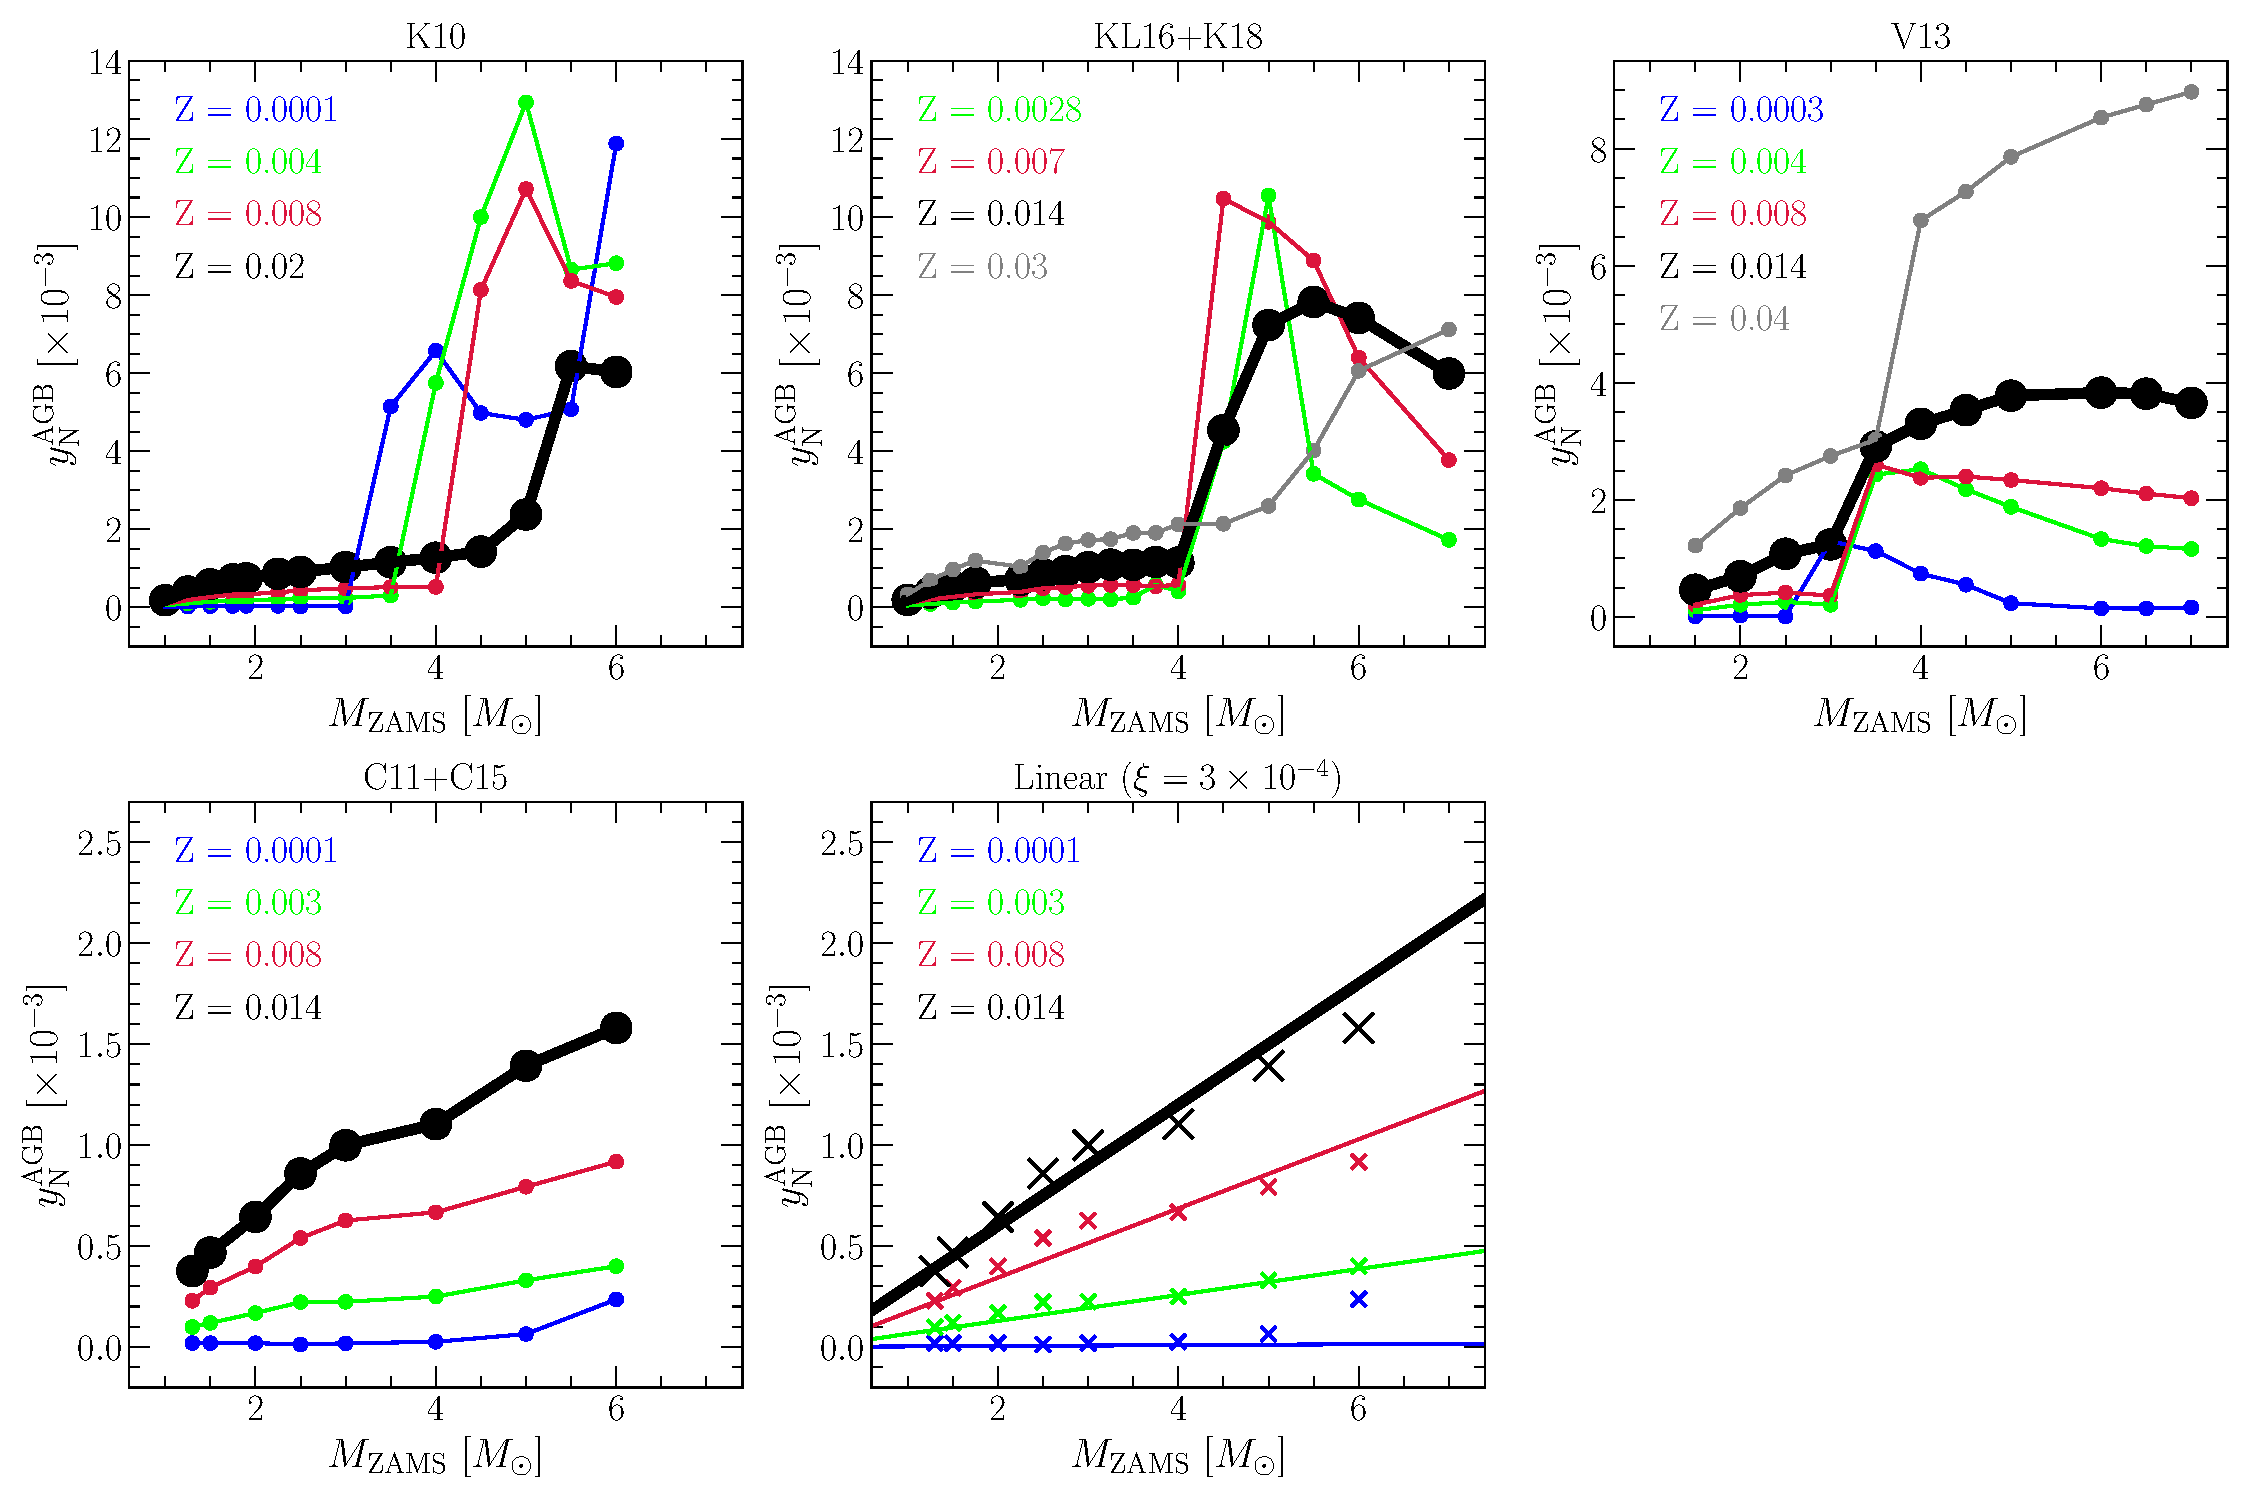
\includegraphics[scale = 0.45]{agb_yield_models.pdf}
\caption{
The fractional yields of N from AGB stars~\yagb{N}~as a function of progenitor
ZAMS mass and birth metallicity~$Z$ as reported by
\citet[][upper left]{Karakas2010},~\citet{Karakas2016} and
\citet[][upper middle]{Karakas2018},~\citet[][upper right]{Ventura2013,
Ventura2014, Ventura2018, Ventura2020}, and~\citet[][lower right]{Cristallo2011,
Cristallo2015}.
For~\citet{Ventura2013, Ventura2014, Ventura2018, Ventura2020} and
\citet{Cristallo2011, Cristallo2015}, we show the yields only for a selection
of metallicities available from their provided tables.
We highlight yields at solar metallicity ($Z = 0.02$ for~\citealp{Karakas2010},
$Z = 0.014$ otherwise) with bold black lines.
In the lower right panel, we show the yields predicted by our linear model
(coloured lines, see equation~\ref{eq:linear_yield}) in comparison to
the~\citet[][coloured X's]{Cristallo2011, Cristallo2015} predictions.
We caution that the axis ranges are not the same between panels in this
figure.
}
\label{fig:agb_yield_models}
\end{figure*}

Here we make use of four previously published tables of AGB star yields
calculated from stellar evolution models, each of which are sampled on a grid
of progenitor masses and metallicities.
To approximate~\yagb{X}~as a smooth function of~$M_\star$ and
$Z_\star$,~\vice~interpolates bi-linearly between grid elements - once in
mass and once in metallicity - and linearly extrapolates above or below in
either quantity as necessary.
By comparing the predicted abundances of the~\citet{Johnson2021} Milky Way
model to the latest observational data, we can constrain how accurately these
``off-the-shelf'' yield models characterize N production.
These models taken from the literature are:
\begin{itemize}
	\item[\textbf{1.}] \citet[][hereafter~\karakasten]{Karakas2010}\footnote{
		We clarify that our abbreviations of these papers (i.e.~\karakasten,
		\karakas,~\ventura, and~\cristallo) refer specifically to their yields
		of N as we adopt them in our model.
		We cite the full names of these papers when referring to their more
		general results.
	} published yields for~$Z = 0.0001$, 0.004, 0.008, and 0.02 progenitors.
	We plot these yields in the upper left panel of 
	Fig.~\ref{fig:agb_yield_models}.

	\item[\textbf{2.}] \citet{Karakas2016} and~\citet{Karakas2018} published
	yields for~$Z = 0.0028$, 0.007, 0.014, and 0.03 progenitors; we hereafter
	refer to these yields as the~\karakas~model.
	We illustrate these yields in the upper middle panel of
	Fig.~\ref{fig:agb_yield_models}.

	\item[\textbf{3.}] We combine the yields for~$Z = 0.0003$ and 0.008
	progenitors from~\citet{Ventura2013} with those at~$Z = 0.004$ from
	\citet{Ventura2014}, at~$Z = 0.014$ from~\citet{Ventura2018}, and at
	$Z = 0.04$ from~\citet{Ventura2020} into a single table of yields.
	In this set, we also include a set of un-published yields at~$Z = 0.001$
	and 0.002 computed from similar models (provided by P. Ventura, private
	communication).
	We hereafter refer to this yield set as the~\ventura~model, and we plot a
	subsample of these yields in the upper right panel of
	Fig.~\ref{fig:agb_yield_models}.

	\item[\textbf{4.}] The default set of AGB star yields in~\vice~is taken
	from~\citet{Cristallo2011, Cristallo2015}, who published yields for
	$Z = 0.0001$, 0.0003, 0.001, 0.002, 0.003, 0.006, 0.008, 0.01, 0.014, and
	0.02 progenitors.
	We hereafter refer to these yields as the~\cristallo~model, and we
	illustrate a subsample of them in the lower left panel of
	Fig.~\ref{fig:agb_yield_models}.
\end{itemize}
\vice~also allows users to construct their own functions of progenitor mass
and metallicity to describe the AGB star yield.
Motivated by the roughly linear nature of the~\cristallo~yields and their
general success once renormalized by a constant factor (see discussion
in~\S~\ref{sec:results:yields}), we construct a model in which the yield is
linearly proportional to both progenitor ZAMS mass and metallicity:
\begin{equation}
\yagb{N} = \xi \left(\frac{M}{M_\odot}\right) \left(\frac{Z}{Z_\odot}\right).
\label{eq:linear_yield}
\end{equation}
We illustrate this model in the lower middle panel of Fig.
\ref{fig:agb_yield_models} for~$\xi = 3\times10^{-4}$ in comparison to
the~\cristallo~yields shown by the coloured X's.
\par
Despite reporting values of the same physical quantities, the N yields
reported by each of these studies show substantial differences between one
another.
Unfortunately, ascertaining the origins of their inconsistencies is difficult
because each model employs its own assumptions for important evolutionary
parameters such as opacity, mass loss, nuclear reaction networks, and
convection and convective boundaries within stars, all of which have a
significant impact on stellar evolution and thus the predicted yields (see
discussion in, e.g.,~\S~5 of~\citealp{Karakas2016}).
However, the differences can be qualitatively understood by considering two
important phenomena known to occur within AGB stars: third dredge-up\footnote{
	Here the time adverbial ``third'' refers only to the fact that these
	dredge-up episodes are occurring while the star is on the asymptotic giant
	branch. Because they are associated with the thermal pulsations of AGB
	stars, there are many episodes of third dredge-up.
} (TDU) and hot bottom burning (HBB).
The variations in how TDU and HBB proceed between different stellar evolution
models arise as consequences of the different input physics.
\par
When an AGB star experiences a thermal pulsation, this is usually accompanied
by a TDU event whereby the convective envelope pentrates into the
hydrogen-depleted core, mixing some of this material with other material
exposed to partial He-shell burning.
This process does not affect N abundances much because at this evolutionary
phase, the core is mostly composed of C and O.
However, the~\Cthirteen($\alpha$, n)\Osixteen~reaction can occur at substantial
rates when the core material is mixed with the He-rich shell.
This reaction is the main source of free neutrons in low mass AGB
stars~\citep{Gallino1998}, and as a consequence, each replenishment of C by TDU
indirectly raises an AGB star's overall yield.
HBB refers to proton capture reactions at the base of the convective envelope,
activating the CNO cycle and producing large amounts of~\Nfourteen~at the
expense of C and O isotopes.
HBB requires a higher mass AGB star progenitor ($M_\text{ZAMS} = 4 - 5~M_\odot$
at~$Z_\odot$ according to~\citealt{Karakas2010}) than TDU
($M_\text{ZAMS} = 2 - 2.5~M_\odot$ at~$Z_\odot$ according to
\citealt{Karakas2010}), but the minimum mass for both decreases at lower
metallicities.
\par
The most efficient N production occurs when both TDU and HBB are active within
an AGB star, because each replenishment of C and O isotopes by TDU adds new
seed nuclei for the CNO cycle with HBB.
This is the reason for the substantial increase in yields at~$\sim$4~\msun~in
the~\karakasten~and~\karakas~models; in both yield sets, every star that
experiences HBB also experiences TDU (see, e.g., Table 1
of~\citealp{Karakas2010}).
Their high mass AGB star yields are higher at low~$Z$ because both HBB and TDU
are more efficient~\citep[][see discussion in]{Ventura2013}.
When the metallicity is low, each TDU episode is deeper due to the lower
opacity, and the base of the convective envelope is hotter, increasing the rate
of CNO cycle reactions in HBB.
% Their high mass AGB star yields depend inversely on metallicity because both
% HBB and TDU are more efficient at low~$Z$ (see discussion in
% \citealp{Ventura2013}).
% For TDU, each penetration by the convective envelope into the core is deeper
% because of the lower opacity.
% For HBB, the base of the convective envelope is hotter, and the rate of CNO
% cycle reactions is an extremely strong function of temperature
% \citep[e.g.][]{Bethe1939}.
This interaction between TDU and HBB is also the reason for the increase in
the~\ventura~yields near~$\sim$3~\msun, but unlike
the~\karakasten~and~\karakas~models, their stars experience both processes only
in this narrow range of mass.
\par
Of all of these yields taken from the literature, the~\cristallo~sample shows
the smoothest dependence on progenitor mass and metallicity.
Below~$\sim$3~\msun, their agreement with the~\karakas~yields is good, but this
model has much lower N yields for higher mass AGB stars.
Even when collapsing the information into TDU and HBB, pinpointing a single
reason for this difference is difficult.
Relative to the~\karakas~yields (see discussion in~\S~5 of
\citealp{Karakas2016}), the~\cristallo~stars have more mass loss, fewer
thermal pulses overall, and weaker HBB due to a lower temperature at the base
of the convective envelope, each of which act to lower the yield of~\Nfourteen.
\par
Although both the~\karakasten~and~\karakas~yield models both show a substantial
increase in N yields above~$\sim$4~\msun, there are some noteworthy differences
between the two.
In the newer version, the yields at solar metallicity are somewhat higher,
and the yields at sub-solar metallicities decreased slightly, particularly for
the highest mass AGB stars.
These differences can be understood by slight variations in the input physics
(A. Karakas, private communication).
A portion of the increase in the yields at solar metallicity can be attributed
to the assumption of~$Z_\odot = 0.02$ versus~$Z_\odot = 0.014$\footnote{
	Changes in the accepted value of the metallicity of the sun trace back to
	the canonical value of~$\sim$2\% derived by, e.g.,~\citet{Anders1989} and
	\citet{Grevesse1998}, later being revised to~$\sim$1.4\% by, e.g.,
	\citet{Lodders2003} and~\citet*{Asplund2005}. See Table 4 of
	\citet{Asplund2009} for a compilation of measured values.
} and the impact this has on both HBB and TDU, but it does not account for the
entire difference.
As a consequence of updates to opacity tables and the adopted solar composition,
the~\karakas~models at solar metallicity are slightly hotter and more compact,
giving them hotter HBB and deeper TDU.
With more thermal pulses overall and therefore a longer AGB lifetime, these
stars have more time to convert~\Ctwelve~into~\Nfourteen.
\karakas~also use low-temperature opacity tables based on~\citet{Marigo2002}
that more closely follow the surface composition of the star.
These opacities are high, making the stars larger and increasing the
mass-loss rate relative to~\karakasten, truncating the N yield of the highest
mass AGB stars.
The~$Z = 0.0028$ model uses the~\citet{Bloecker1995} mass-loss prescription
rather than that of~\citet{Vassiliadis1993}, which was used for
the~\karakasten~yields as well as the yields at other metallicities in
the~\karakas~model.
This choice results in fewer thermal pulses and a shorter AGB lifetime, giving
them less time to process C and O nuclei into~\Nfourteen.
\par
In the interest of consistency, when we adopt a particular AGB star yield model
for N, we also adopt the corresponding table within~\vice~for O and Fe when
possible.\footnote{
	In the case of~\citet{Ventura2013, Ventura2014, Ventura2018, Ventura2020},
	AGB star yields of Fe are not available, and our linear model is only
	appropriate for N.
	In these cases, we assume the~\vice~default of the~\citet{Cristallo2011,
	Cristallo2015} yields for both O and Fe.
}
These O and Fe yields, however, are negligible compared to their SN yields.
Although we focus our investigation on AGB yields from~$\lesssim$~7~\msun stars,
slightly more massive stars (up to~$\sim$12~\msun) sit near the critical mass
boundaries between different types of massive white dwarfs and electron capture
SN progenitors.
\citet{Doherty2017} investigated theoretically predicted yields of these stars
and found significant production of CNO isotopes.
There is also the intriguing possibility of the CNO yields from the earliest,
most metal-poor AGB stars (e.g. the~$Z = 10^{-5}$ models
of~\citealp{Gil-Pons2013, Gil-Pons2021}) and the insight this may afford into
N production at low~$Z$ and the most metal-poor stars in the Galaxy.
While experiments with such yields in our GCE models would be interesting, this
is beyond the scope of the current paper since our AGB yield models already
span a wide range of assumptions regarding stellar evolution.



\subsection{IMF-Averaged AGB Star Yields: Metallicity and Time Dependence}
\label{sec:yields:imf_agb}

% fig 4
\begin{figure*}
\centering
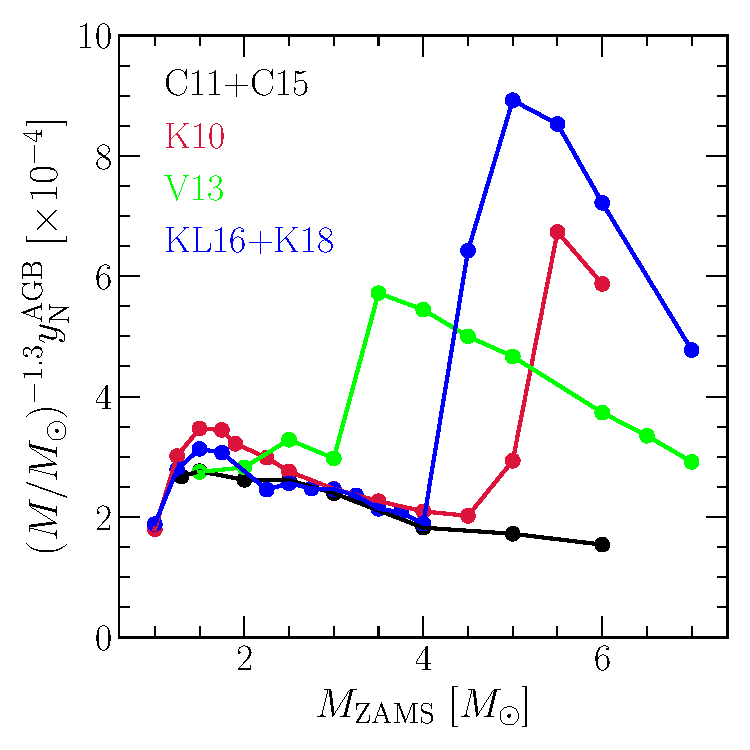
\includegraphics[scale = 0.46]{agb_yield_models_imfweighted.pdf}
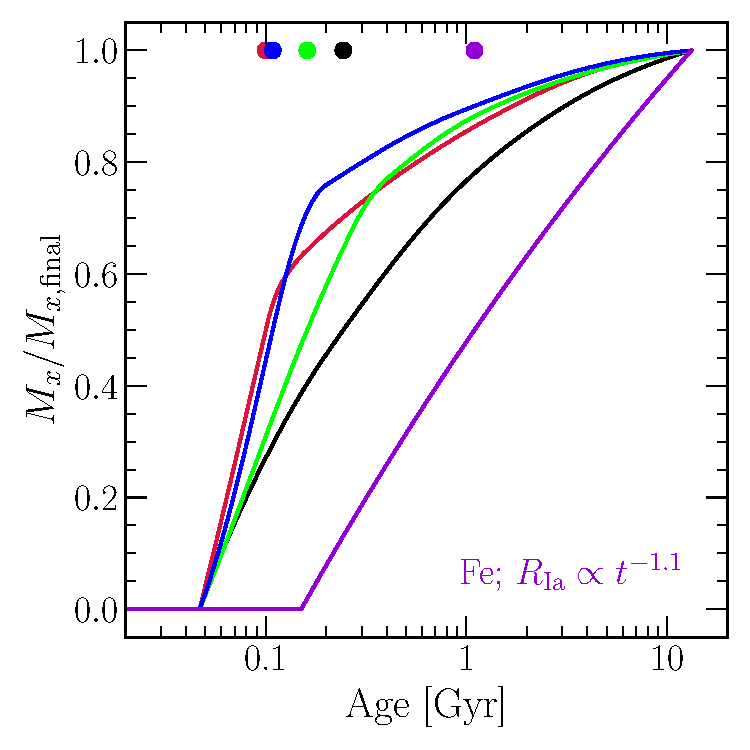
\includegraphics[scale = 0.45]{ssp_production_modelcomp.pdf}
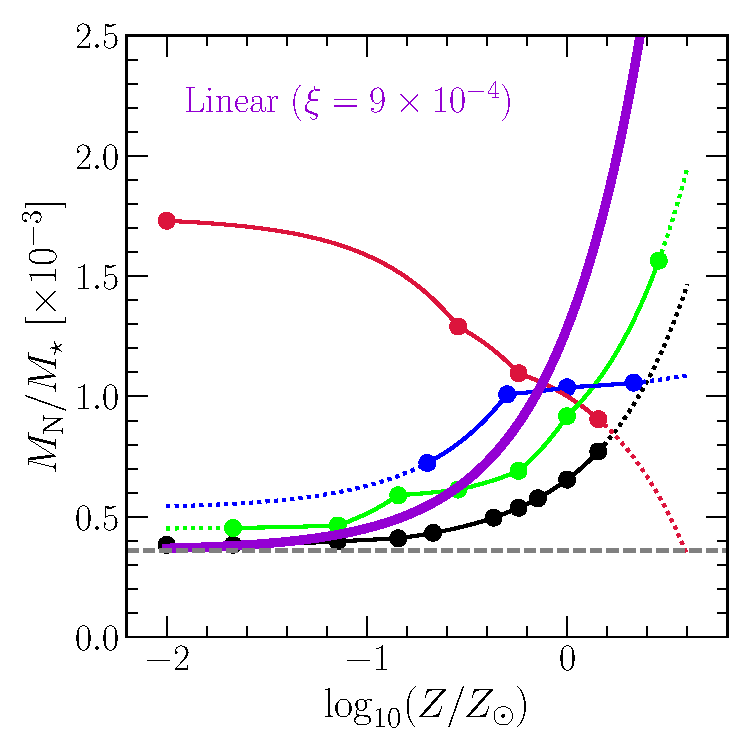
\includegraphics[scale = 0.46]{ssp_production_metdep.pdf}
\caption{
\textbf{Left}: The IMF-weighted mass yield of N from AGB stars as a function of
progenitor ZAMS mass at solar metallicity ($Z = 0.02$ in~\karakasten,
$Z = 0.014$ otherwise).
\textbf{Middle}: The net mass of N produced by AGB stars from a single stellar
population for each of our yield models at solar metallicity.
The purple line denotes the same for Fe assuming our~$t^{-1.1}$ DTD as in the
\citet{Johnson2021} chemical evolution model.
All values are normalized to the total mass produced at an age of 13.2 Gyr.
Points at the top of the panel denote the ages at which 50\% of the total mass
yield has been produced.
\textbf{Right}: The total amount of N produced by a 13.2 Gyr old stellar
population as a function of metallicity for each of our yield models normalized
by the stellar population's initial mass.
Points mark metallicities at which the published tables report yields.
}
\label{fig:ssp}
\end{figure*}

To more directly compare these AGB star yields predicted from stellar
evolution models, we plot their IMF-weighted yields at solar metallicity
($Z = 0.02$ for~\karakasten, $Z = 0.014$ otherwise) in the left hand panel of
Fig.~\ref{fig:ssp}.
As mentioned in~\S~\ref{sec:yields:agb}, the AGB star yield~\yagb{N}~as we
have parameterized it is in units of the progenitor star's ZAMS mass, and
consequently the~\textit{mass yield} of N is given by~$M_\star \yagb{N}$.
With an additional weight of~$M_\star^{-2.3}$ from the IMF in this mass range
\citep[e.g.][]{Kroupa2001}, we therefore multiply the values of~\yagb{N}~by
$(M_\star / M_\odot)^{-1.3}$ to quantify a star's relative contribution to the
total N yield taking into account the intrinsic mass distribution.
Even with the additional weight of~$M_\star^{-1.3}$, the~\cristallo~yields are
relatively mass-independent.
For the other yield models, the contributions from higher mass AGB stars is
yet more pronounced due to the effects of TDU and HBB discussed
in~\S~\ref{sec:yields:agb}.
\par
Using~\vice's~\texttt{vice.single\_stellar\_population} function, in the
middle panel of Fig.~\ref{fig:ssp} we plot the total N yield as a function of
age from a single stellar population.
For the sake of this calculation, we set all CCSN yields of N to zero in order
to highlight the AGB star contribution.
We show the results of this procedure for solar metallicity only (again
$Z = 0.02$ for~\karakasten,~$Z = 0.014$ otherwise), and we normalize all values
to the total mass produced at~$T = 13.2$ Gyr (the total amount of time our GCE
model is integrated over; see discussion in~\S~\ref{sec:multizone}).
% \par
Under the~\cristallo~yields, it takes~$\sim$250 Myr for a single stellar
population to produce~$\sim$50\% of its N from AGB stars, as noted by the
coloured points at the top of the panel.
This is in good agreement with~\citet{Maiolino2019}, who find that similar
parameter choices predict 80\% of the N yield to be ejected within~$\sim$1 Gyr
(see their Fig 1).
The characteristic timescales for N production are even shorter in our alternate
yield models with more pronounced contributions from massive stars due to
their short lifetimes~\citep[e.g.][]{Larson1974, Maeder1989, Padovani1993}.
For comparison, we plot the enrichment of Fe by our~$t^{-1.1}$ power-law DTD,
also with the CCSN yield set to zero to highlight the delayed component.
The characteristic delay time for Fe production is considerably longer than
that of N - up to an order of magnitude depending on which yield model is
adopted.
As noted in~\citet{Johnson2021}, a characteristic delay time of~$\sim$1 Gyr
is exactly as expected for a~$\sim t^{-1}$ DTD because half of the SN Ia
events occur between 100 Myr and 1 Gyr and the other half between 1 Gyr and
10 Gyr.
\par
A characteristic delay time of only~$\sim$250 Myr may seem surprising given
the relatively mass-independent nature of the IMF-weighted~\cristallo~yields.
This arises out of the steep nature of the stellar mass-lifetime relation
\citep[e.g.][]{Larson1974, Maeder1998, Padovani1993}.
For example, 2 and 3~\msun~stars live only~$\sim$1.2 Gyr and~$\sim$400 Myr,
respectively, and over the course of 13.2 Gyr, only stars of masses
$\gtrsim$0.9~\msun~will have enough time to finish their hydrogen burning.
Consequently, most of the mass range of stars that will evolve through an
AGB phase will do so within the first few hundred Myr after their formation,
and with mass-independent IMF-weighted yields, this accounts for most of the
N.
We clarify that this characteristic delay time applies~\textit{only} to N and
not to other elements produced by AGB stars.
As we have illustrated here, the effective DTD of AGB star enrichment is
dictated by the combination of the stellar mass-lifetime relation and the
mass dependence of the yield, which should in principle differ from element to
element.
Other elements produced by slow neutron capture often have the highest yields
from lower mass AGB stars (e.g. strontium, for which the yields as
reported by~\citealp{Cristallo2011, Cristallo2015} are dominated by
$M_\text{ZAMS} = 2 - 3~\msun$ progenitors; see Fig. 5 of
\citealp{Johnson2020}).
The characteristic delay-times will be as long as a few Gyr if and only if the
yields are dominated by~$\lesssim$2~\msun~stars.
We caution against interpretations of AGB star nucleosynthesis which attribute
a single characteristic delay time to this enrichment channel as this is
likely only accurate for order of magnitude estimates.
\par
In the right panel of Fig.~\ref{fig:ssp}, we plot the total amount of N
produced by a 13.2 Gyr old single stellar population as a function of its
initial metallicity according to all of our AGB star yield tables, including
the linear model (see equation~\ref{eq:linear_yield} and discussion
in~\S~\ref{sec:yields:agb}).
For this calculation, we include the CCSN yield ($\ycc{N} = 3.6\times10^{-4}$;
see discussion in~\S~\ref{sec:yields:ccsne}).
In general, there is good qualitative agreement between the~\cristallo~and
the~\ventura~models, the only major difference being the normalization.
The predictions with the linear model with~$\xi = 3\times10^{-4}$ are nearly
identical to the~\cristallo~model, which is unsurprising given their
similarity in Fig.~\ref{fig:agb_yield_models}.
The value at which these N yields flatten off at low~$Z$ is reflective of our
adopted value of~\ycc{N}.
Up to~$\log_{10}(Z / Z_\odot) \approx -0.2$, the~\karakas~yields predict a
similar trend as~\cristallo~and~\ventura, also with a difference in
normalization, but at solar and super-solar metallicities they predict much
more metallicity-independent N yields than others.
The~\karakasten~yields, on the other hand, do not agree with any of the other
models, instead predicting N yields to~\textit{decrease} monotonically with
increasing~$Z$.
These differences between the~\karakasten~and~\karakas~models trace back to
differences regarding the opacity and mass loss prescriptions (see discussion
in~\S~\ref{sec:yields:agb}).
Although the normalization depends on the SN yields of all elements, we
demonstrate in~\S~\ref{sec:results:yields} that reproducing the~\ohno~relation
as observed requires N yields which scale roughly linearly with metallicity as
in the~\cristallo~and~\ventura~models.

\end{document}

